\documentclass[10pt,a4paper]{article}
\usepackage[utf8]{inputenc}
\usepackage{amsmath}
\usepackage{amsfonts}
\usepackage{amssymb}
\usepackage{makeidx}
\usepackage{graphicx}
\usepackage[left=2cm,right=2cm,top=2cm,bottom=2cm]{geometry}
\author{Jiménez Cortés Raúl}

\begin{document}
\begin{center}
\begin{LARGE}
\textbf{INGENIERÍA MECATRÓNICA}\\
\end{LARGE}
{\large Sistemas Eletrónicos De Interfaz}\\
\begin{figure}[hbtp]
\centering

\includegraphics[scale=0.80]{UPZMG_Mecatr_nica.png}
\end{figure} 
\begin{center}
\begin{LARGE}
EV-2-8-Calcular Los Parametros De Un Circuito De Activacion De Transitores De Potencia.
\end{LARGE}
\end{center}

\begin{Large}
\textbf{Alumno}
\\\textit{Raúl Jiménez Cortés}
\textbf{\\Maestro}
\\\textit{Morán Garabito Carlos Enriquez}
\textbf{\\Fecha de Entrega}
\\\textit{29/10/2019}
\textbf{\\Grupo}
\\\textit{4º "B"}
\end{Large}
\end{center}

\newpage
\section{Transitores De Potencia}
\textbf{Caracteristicas}\\
-Ic corriente máxima de colector (o drenador)\\
-Uceo tensión de ruptura colector – emisor (o drenador  - surtidor) con la base (o puerta) abierta\\
-Ucesat  tensión de saturación colector- emisor (o drenador  - surtidor)\\
-Pmax  potencia máxima disipable en régimen continuo.\\
Básicamente, las características de los transistores de potencia dependen del tipo de transistor, del semiconductor y de la fabricación. Se emplean en germanio (bipolares de baja tensión), principalmente de silicio y, solo para transistores FET especiales para amplificadores de comunicación. Lo más común en fabricación es la difusión. La velocidad de conmutación es grande y se emplean en convertidores cd-cd y cd-ca con diodos conectados en paralelo inverso para proporcionar flujo bidireccional de corriente se emplean en aplicaciones de baja a mediana potencia.\\
Los transistores de potencia se clasifican en 3 categorías que son las siguientes:\\
-Transistores bipolares de unión (BJT)\\
-Transistores  Efecto de campo (FET)\\
-Transistores bipolares de compuerta aislada  (IGBT).\\
\textbf{Transistores bipolares de unión (BJT)}\\
se forman agregando una segunda región p o n a un diodo de union pn. Con dos regiones n y una p, se forman dos uniones, teniéndose asi un transistor NPN, y con dos regiones p  y una n, se forma un transistor PNP, como se ve en la figura posee tres terminales (colector,  emisor y base).\\

\begin{center}
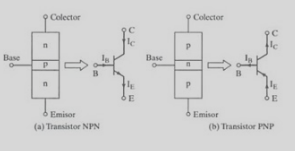
\includegraphics[scale=0.8]{1.png}
\end{center} 

\textbf{El transistor bipolar tiene dos uniones}\\
la unión colector – base (CBJ) y la unión base – emisor (BEJ).Hay dos regiones n+  para el emisor del transistor NPN, dos regiones  p+ para el emisor de transistor PNP [Secciones transversales de un BJT]

Hay tres configuraciones: colector comun, base comun y emisor comun. La de emisor comun de NPN es la que se usa mayormente en conmutaciones. Para un transistor PNP se invierten las polaridades de todas las corrientes y voltajes.\\

\begin{center}
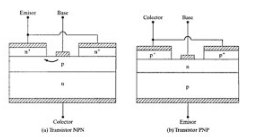
\includegraphics[scale=0.8]{2.png}
\end{center} 

\textbf{Un transistor opera en tres regiones:}\\
\textbf{Region de corte:} el transistor esta abierto o apagado, la corriente de base no es suficiente para saturarlo, y las dos uniones estan polarizadas inversamente.\\
\textbf{Region activa:}el transistor actua como un amplificador, en el que la corriente de base se amplifica una ganacia determinada, y el voltaje colector – emisor disminuye al aumentar la corriente de base. La union colector – base (CBJ) esta polarizada inversamente y la union colector – emisor (BEJ) esta polarizada directamente.\\
\textbf{Region de saturacion:}la corriente de base es suficientmente alta como para que el voltaje colector – emisor sea bajo, y el transistor actua como un interruptor. Las dos uniones (CBJ y BEJ) tienen polarizacion directa.\\ 
\textbf{Transistores  Efecto de campo (FET)}\\
El transistor de efecto campo (Field-Effect Transistor o FET, en inglés) es en realidad una familia detransistores que se basan en el campo eléctrico para controlar la conductividad de un "canal" en un material semiconductor. Los FET pueden plantearse como resistencias controladas por diferencia de potencial.\\

\begin{center}
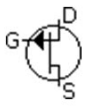
\includegraphics[scale=0.8]{3.png}
\end{center} 

El transistor de efecto campo (Field-Effect Transistor o FET, en inglés) es en realidad una familia detransistores que se basan en el campo eléctrico para controlar la conductividad de un "canal" en un material semiconductor. Los FET pueden plantearse como resistencias controladas por diferencia de potencial.\\

\begin{center}
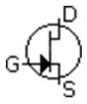
\includegraphics[scale=0.8]{4.png}
\end{center} 

Tienen tres terminales, denominadas puerta (gate), drenador (drain) y fuente (source). La puerta es la terminal equivalente a la base del BJT. El transistor de efecto de campo se comporta como un interruptor controlado por tensión, donde el voltaje aplicado a la puerta permite hacer que fluya o no corriente entre drenador y fuente.\\
Las imágenes son Símbolos esquemáticos para los JFETs canal-n y canal-p. G=Puerta(Gate), D=Drenador(Drain) y S=Fuente(Source).) 1- P-chanel. 2 - N-channel.

El Funcionamiento Del Transistor de efecto de campo es distinto al del BJT. En los MOSFET, la puerta no absorbe corriente en absoluto, frente a los BJT, donde la corriente que atraviesa la base, pese a ser pequeña en comparación con la que circula por las otras terminales, no siempre puede ser despreciada. Los MOSFET, además, presentan un comportamiento capacitivo muy acusado que hay que tener en cuenta para el análisis y diseño de circuitos.

Así como los transistores bipolares se dividen en NPN y PNP, los de efecto de campo o FET son también de dos tipos: canal n y canal p, dependiendo de si la aplicación de una tensión positiva en la puerta pone al transistor en estado de conducción o no conducción, respectivamente. Los transistores de efecto de campo MOS son usados extensísimamente en electrónica digital, y son el componente fundamental de los circuitos integrados o chips digitales.\\
\textbf{ Características}\\
-Tiene una resistencia de entrada extremadamente alta (casi 100M).\\
-No tiene un voltaje de unión cuando se utiliza Conmutador (Interruptor).\\
-Hasta cierto punto es inmune a la radiación.\\
-Es menos ruidoso.\\
-Puede operarse para proporcionar una mayor estabilidad térmica.\\
 La sigla IGBT corresponde a las iniciales de isolated gate bipolar transistor o sea transistor bipolar de puerta de la salida.

El IGBT es un dispositivo semiconductor de potencia híbrido que combina los atributos del TBJ y del MOSFET. Posee una compuerta tipo MOSFET y por consiguiente tiene una alta impedancia de entrada. El gate maneja voltaje como el MOSFET. El símbolo más comúnmente usado se muestra en la figura . Al igual que el MOSFET de potencia, el IGBT no exhibe el fenómeno de ruptura secundario como el TBJ.

El transistor bipolar de puerta aislada (IGBT) es un dispositivo electrónico que generalmente se aplica a circuitos de potencia.

Este es un dispositivo para la conmutación en sistemas de alta tensión. La tensión de control de puerta es de unos 15V. Esto ofrece la ventaja de controlar sistemas de potencia aplicando una señal eléctrica de entrada muy débil en la puerta.
El IGBT de la figura es una conexión integrada de un MOSFET y un BJT. El circuito de excitación del IGBT es como el del MOSFET, mientras que las características de conducción son como las del BJT. El IGBT es adecuado para velocidades de conmutación de hasta 20 KHz y ha sustituido al BJT en muchas aplicaciones.\\
\textbf{Simbologia}\\
Es un componente de tres terminales que se denominan GATE (G) o puerta, COLECTOR (C) y EMISOR (E) y su símbolo corresponde al dibujo de la figura siguiente.
Su estructura microelectrónica es bastante compleja es por ello que lo describimos en base a su esquema equivalente

\begin{center}
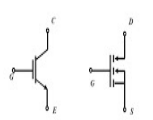
\includegraphics[scale=0.8]{5.png}
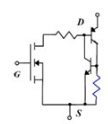
\includegraphics[scale=0.8]{6.png}
\end{center} 


\textbf{Curva característica IGBT:}\\

\begin{center}
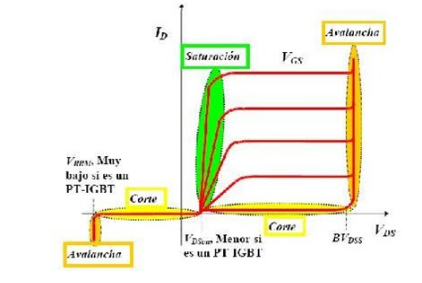
\includegraphics[scale=0.8]{7.png}
\end{center} 

\textbf{Caracteristica}\\
-IDmax Limitada por efecto Latch-up.\\
-VGSmax Limitada por el espesor del óxido de silicio.\\
-Se diseña para que cuando VGS = VGSmax la corriente de cortocircuito sea entre 4 a 10 veces la nominal (zona activa con VDS=Vmax) y pueda soportarla durante unos 5 a 10 956;s. y pueda actuar una protección electrónica cortando desde puerta.\\
-VDSmax es la tensión de ruptura del transistor pnp. Como 945; es muy baja, será  VDSmax=BVCB0 Existen en el mercado IGBTs con valores de 600, 1.200, 1.700,  2.100 y 3.300 voltios. (anunciados de 6.5 kV).\\
-La temperatura máxima de la unión suele ser de 150ºC (con SiC se esperan  valores mayores)
-Existen en el mercado IGBTs encapsulados que soportan hasta 400 o 600 Amp.\\
-La tensión VDS apenas varía con la temperatura 8658; Se pueden conectar en  paralelo fácilmente 8658; Se pueden conseguir grandes corrientes con facilidad,  p.ej. 1.200 o 1.600 Amperios.\\
-En la actualidad es el dispositivo mas usado para potencias entre varios kW y un  par de MW, trabajando a frecuencias desde 5 kHz a 40kHz.\\

\section{Como Se Calcula Los Parametros De Potencia En Los Transitores}
En esta se mostraran unos ejercicios con las formulas el cual da en como calcular el transitor de sus parametros en su potencia.
\begin{center}
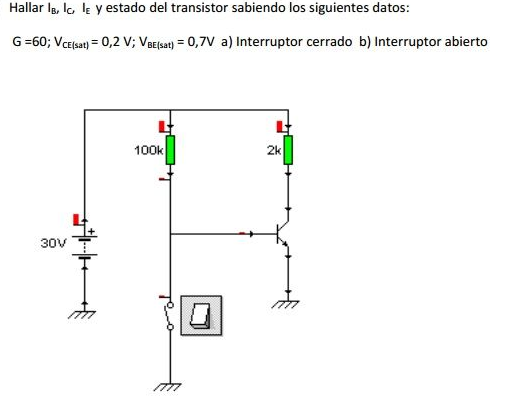
\includegraphics[scale=0.8]{8.png}
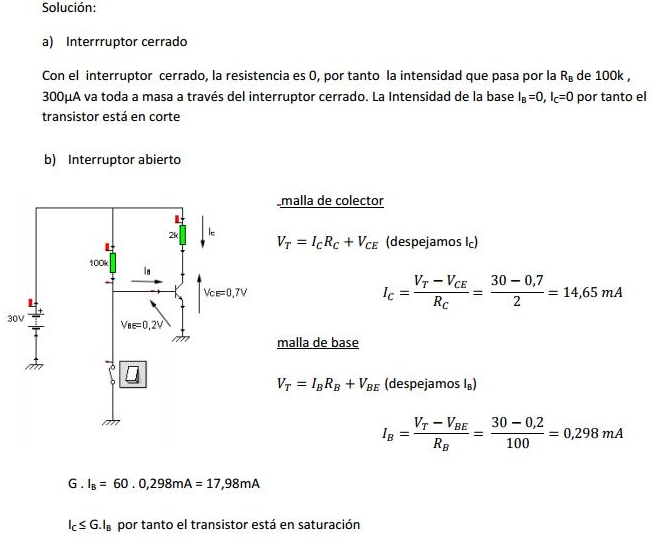
\includegraphics[scale=0.6]{9.png}
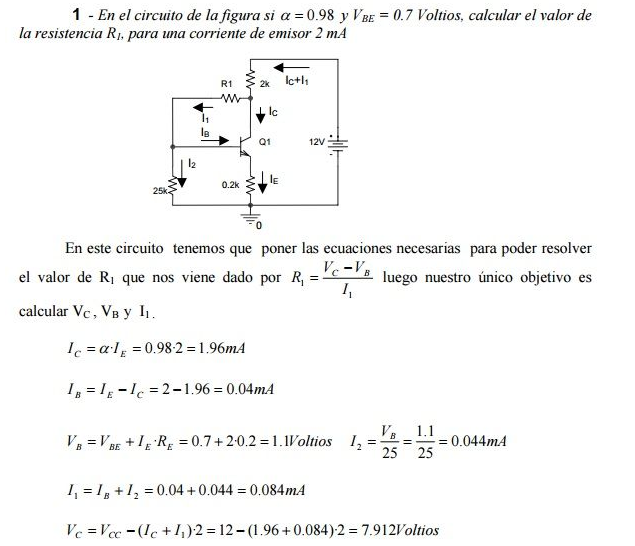
\includegraphics[scale=0.8]{10.png}
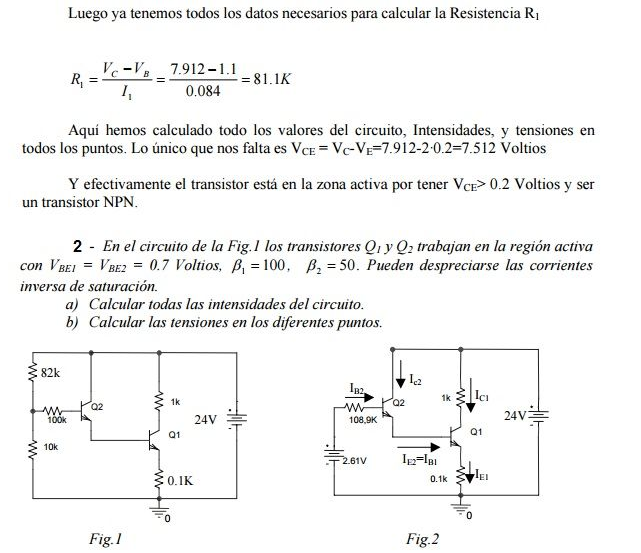
\includegraphics[scale=0.8]{11.png}
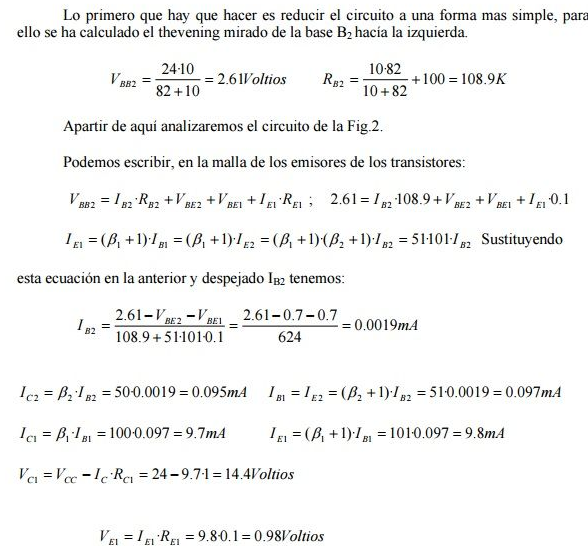
\includegraphics[scale=0.8]{12.png}
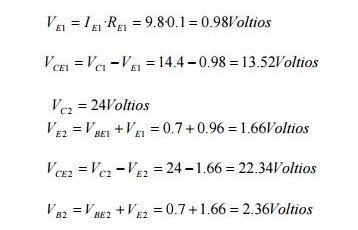
\includegraphics[scale=0.8]{13.png}
\end{center}


\bibliography{tarea7.bib}{}
\bibliographystyle{plain}{https://www.areatecnologia.com/electronica/ejercicios-transistores.html\\https://sites.google.com/site/transistoresfototransistores/classroom-news}

\end{document}